% 93-26(93쪽) — 두 직선 $y=x$, $y=\dfrac{1}{3}x$ 가 이루는 예각 θ(원문 「오른쪽 그림」). 스캔 화질이 낮아 TikZ 로 다시 그림.
% 라벨은 원문 것만: $x$, $y$, O, 두 직선의 이름, 각 θ. cos θ 의 값(답)은 그림에 적지 않는다.
\begin{tikzpicture}[line width=0.6pt, x=0.52cm, y=0.52cm, >=stealth]
  \draw[->, line width=0.7pt] (-1.25,0) -- (4.05,0) node[below=1pt] {$x$};
  \draw[->, line width=0.7pt] (0,-0.70) -- (0,4.15) node[left=1pt] {$y$};
  \draw (-0.95,-0.95) -- (3.25,3.25);
  \draw (-1.15,-0.383) -- (3.85,1.283);
  \draw[line width=0.45pt] ([shift={(18.43:1.00)}]0,0) arc [start angle=18.43, end angle=45, radius=1.00];
  \node[font=\small, anchor=north west] at (0.02,-0.06) {$\pt{O}$};
  \node[font=\small, anchor=south east] at (3.30,3.18) {$y=x$};
  \node[font=\small, anchor=south west] at (2.45,1.42) {$y=\dfrac{1}{3}x$};
  \node[font=\small] at (1.32,0.74) {$\theta$};
\end{tikzpicture}
